\chapter{АНАЛІЗ ПРЕДМЕТНОЇ ОБЛАСТІ\\ТА ПОСТАНОВКА ЗАДАЧІ}

\section{Поняття вокселя та воксельних структур даних}

\textbf{Воксель} \engl{volume $+$ pixel} --- одиничний елемент \textit{воксельного} простору, що являє собою решітку з елементів фіксованого розміру. У тривимірному простору є аналогом пікселя у двовимірному. У процесі трасування променів він грає роль як \textit{візуального елемента}, оскільки 3D моделі у даному проєкті будуть самі будуть складатися з фіксованої сітки вокселів, так і \textit{логічного елемента}, так як воксель є частиною загального воксельного об'єма (World Volume), який буде використовуватися у відкладеному рендерингу. \cite{wiki:voxel}

\begin{figure}[ht]
    \centering
    \input{figures/voxel_model}
    \caption\centering{Воксельна модель дерева, представлена у\\вигляді тривимірного масиву вокселів.}
    \label{fig:voxel}
\end{figure}

Найпростішою формою представлення воксельного об'єму є однорідний \textbf{тривимірний масив}. Це масив розміру $N \times M \times P$, де $N, M, P$ --- це розміри обмежувальної коробки воксельної моделі. У реалізації в шейдерній мові він може бути представлений у вигляді лінійного масиву, індекс якого за координатами $x, y, z$ буде рахуватися за формулою: $x + y \times N + z \times N \times M$; або ж у вигляді 3D-текстури, з якою можна працювати за допомогою вбудованої функції $\operatorname{textureLoad}(x, y, z, L)$, де $L$ --- це MIP-рівень, який ми пізніше використаємо для подальшої оптимізації. 

Однією із більш просунутих структур даних для зберігання воксельного об'є\-му є \textbf{октодерево} \engl{octree} --- дерево, в якому кожен вузол має рівно вісім нащадків і представляє собою кубічний об'єм простору, який розділяється на вісім менших кубів при досягненні певного критерію розбиття; в нашому випадку --- якщо цей об'єм рекурсивно містить хоча б один ``твердий'' воксель. Octree дозволяє ефективно зберігати та обробляти великі об'єми даних, оскільки дозволяє зберігати інформацію лише про ті частини простору, які містять важливі дані, і пропускати порожні області. \cite{sparseOctrees}

Однак, для оптимізації пам'яті використання октодерева на GPU є нелегкою задачею через відсутність у шейдерних мовах вказівників, щоб не зберігати порожні області воксельного об'єму у пам'яті. Проте в цій роботі для зберігання воксельного об'єму буде використана 3D текстура з MIP-рівнями, що дозволить принаймні оптимізувати прохід по воксельному об'єму за допомогою рівнів октодерева.

\textbf{Вокселізацією} називається процес перетворення будь-яких тривимірних даних (сфера, задана формулою, меш 3D моделі) у дискретне (воксельне) представлення. Також вокселізацією можна назвати перетворення воксельних \linebreak об'ємів, що не вирівняні за воксельною сіткою; наприклад, до яких застосована трансформація (зміщення, поворот, масштаб). Такий процес ще називається мапуванням \engl{mapping}, подібно до мапування у 2D зображеннях.

\section{Основи трасування променів}
\textbf{Трасування променів} --- це процес відстеження шляху від уявного ока (камери) через кожен піксель області перегляду \engl{Viewport} та обчислення кольору видимого (на який падає промінь) об'єкта, враховуючи навколишнє середовище, джерела світла, фізичні властивості матеріалу об'єкта тощо.

\begin{figure}[ht]
    \centering
    \begin{tikzpicture}[font=\sffamily]
    % Screen
    \foreach \x in {0,1,2,3,4,5} {
        \foreach \y in {0,1,2,3,4,5} {
            \draw (3,\x*0.5,\y*0.5) -- ++(0,0.5,0) -- ++(0,0,0.5) -- ++(0,-0.5,0) -- cycle;
        }
    }
    \node at (-2,11.5) {Область перегляду};  

    % Camera
    \cubesurface{0}{0}{1}{1}{white};
    \draw (-1.3,4.5) ellipse (0.15cm and 0.3cm);
    \node at (-3.5,7) {Камера};  

    % Shadow
    \fill[lightgray] (7.5,0) ellipse (2cm and 1.5cm);

    % Ball
    \shade[ball color=gray, shading angle=270] (8,1.5) circle (1.5cm);
    \node at (12.5, -2) {Об'єкт сцени};  

    % Sun
    \foreach \angle in {15,60,105,150,195,240,285,330} {
        \draw (6,8) -- ++(\angle:1.2cm);
    }
    \draw[fill=yellow] (6,8) circle (0.6cm);
    \node at (8,9.5) {Джерело світла};  

    % Rays
    \draw[-stealth, thick, blue] (-1.3,4.5) -- (6,3.5);
    \draw[-stealth, thick, blue] (-1.3,4.5) -- (6.3,4.5);
    \draw[-stealth, thick, blue] (-1.3,4.5) -- (8,-1);
    \node[blue] at (3.5, 5.5) {Промінь погляду};  

    \draw[thick, orange] (8,-1) -- (7.5,1.25);
    \draw[-stealth, thick, orange] (7,3.5) -- (6,8);
    \node[orange] at (8.5, 5) {Промінь тіні};  
\end{tikzpicture}
    \caption\centering{Діаграма трасування променів.}
    \label{fig:ray_tracing}
\end{figure}

Загальне трасування променів є потужним методом рендерингу, який дозволяє досягти високої якості зображення шляхом моделювання фізичних явищ, що відбуваються при взаємодії світла з об'єктами. Цей підхід включає в себе не лише базове трасування променів для визначення видимості об'єктів, але й складніші техніки, такі як обчислення тіней, відбиттів та заломлень. Основна ідея загального трасування променів полягає в тому, щоб відстежувати шлях променів світла від джерел до камери, враховуючи всі можливі взаємодії з об'єктами на сцені. Це дозволяє створювати реалістичні зображення, які враховують не лише геометрію об'єктів, але й їх матеріали, освітлення та інші параметри сцени на об'єктів.

\begin{figure}[ht!]
    \centering
    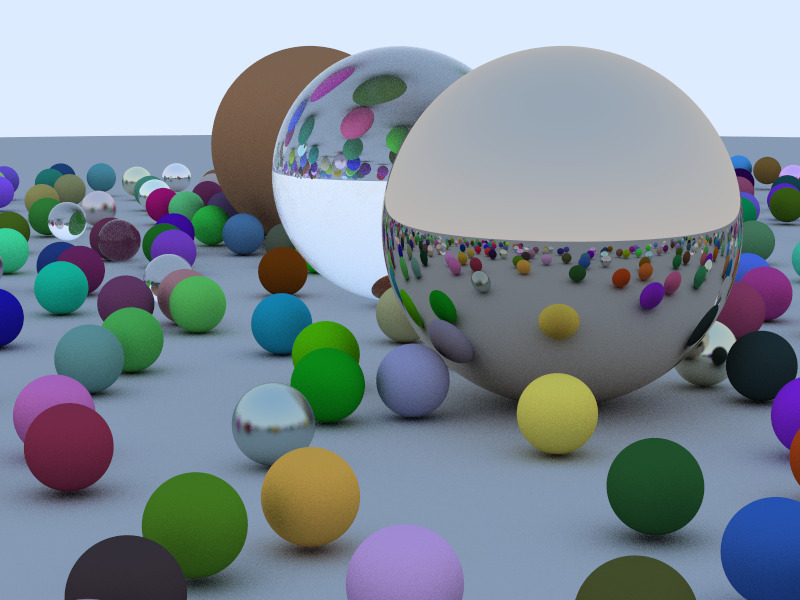
\includegraphics[width=0.4\textwidth]{figures/ray_tracing_one_weekend.jpeg}
    \caption\centering{Приклад трасування променів для сфер на площині\cite{RayTracingInOneWeekend}.}
    \label{fig:ray_tracing_example}
\end{figure}

Програмно трасувальник променів кидає промінь від кожного пікселя, який проходить через кожен об'єкт на сцені за один прохід рендерингу, а потім відображає результат на площині розміром з область перегляду, що являє собою комбінацію двох растеризованих трикутників. Сам \textit{промінь} --- це структура даних, яка складається з \textbf{точки початку} і \textbf{вектору напрямку}. При повторному відбиванню променів від поверхні, точкою початку наступного променя стає точка перетину променя з об'єктом.

\subsection{Основні проблеми реалізації алгоритму трасування променів}
Під час реалізації наївного алгоритму рей трейсингу, основними проблемами, з якими можна зіткнутися:

\begin{enumerate}[itemsep=0pt, topsep=0pt]
    \item \textbf{``Тіньове акне''} \engl{shadow acne}. Це типова проблема, яка з'явля\-ється під час трасування променів для тіней, навколишнього перекриття \engl{ambient occlusion, AO} та інших видів затінення, коли промінь відбивається від поверхні об'єкта і перетинає сам себе, оскільки його точка початку знаходиться під поверхнею, що зумовлене проблемою точності обрахунків чисел з рухомою комою. Простий та ефективний метод вирішення даної проблеми --- це додавання невеликого відступу від поверхні об'єкта сцени вздовж нормалі даної поверхні до точки початку променя.
    \item \textbf{``Екстремальне'' тіньове акне}. Воно виникає під час трасування променів у воксельному просторі, коли вокселі вокселізованого об'єкта сцени ``випирають'' з-під самого об'єкту, перетинаючи його поверхню, що створює артефакти, подібні до звичайного тіньового акне. Так само, як і для звичайного тіньового акне, можна використати відступ вздовж нормалі, однак для великих розмірів одиничного вокселя це не дасть значного ефекту, а при збільшенні цього відступу точність затінення буде зменшуватися. Тому окрім відступу вздовж нормалі поверхні, точка початку променя додатково зміщується у напрямку самого променя на частку розміру вокселя. Такий зсув гарантує, що початок трасування знаходиться не лише поза геометрією об'єкта, але й поза граничною площиною вокселя, усуваючи ситуацію, коли перший крок DDA-алгоритму потрапляє в той самий воксель.
    \begin{figure}[ht!]
        \centering
        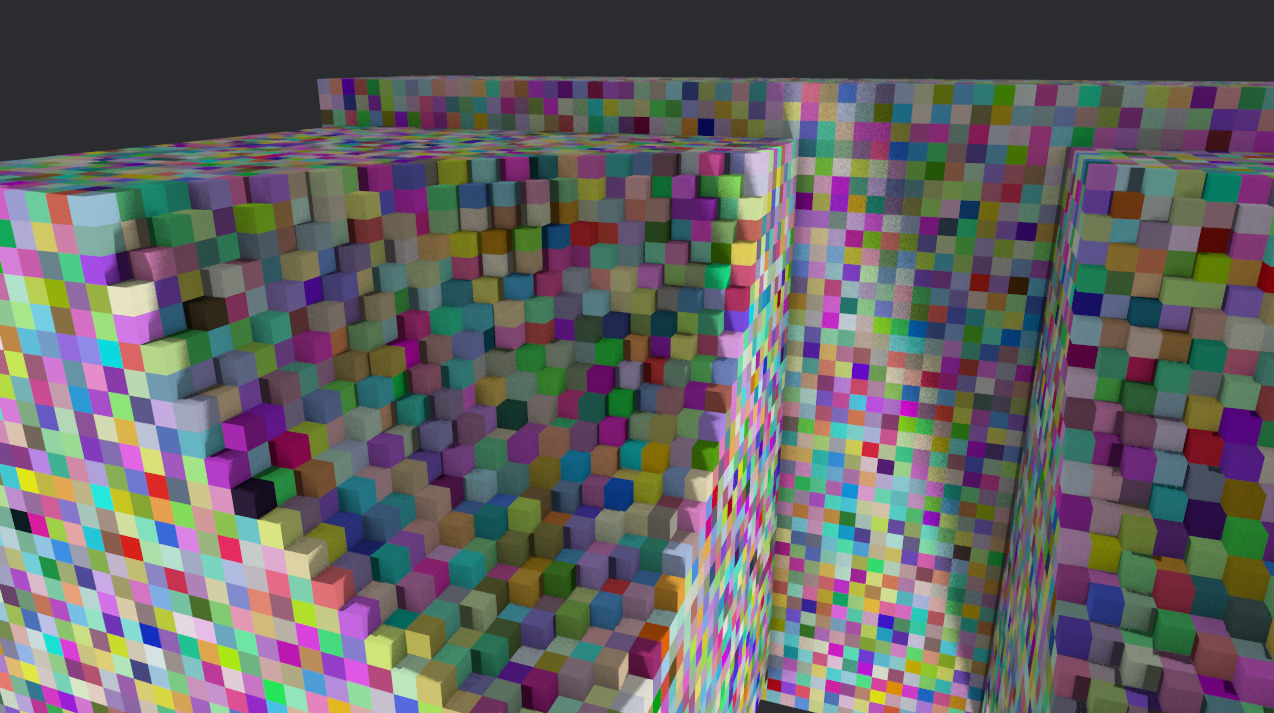
\includegraphics[width=0.7\textwidth]{figures/extreme_acne.jpeg}
        \caption\centering{Екстремальне тіньове акне в орієнтованому воксельному об'ємі.}
        \label{fig:ray_tracing_example}
    \end{figure}
    \item \textbf{Перекривання об'єктів}. При неправильній роботі з буфером глибини (Z-буфер), дані попередньо відтрасованих об'єктів перезаписуються незалежно від того, чи об'єкт знаходиться ближче до камери, чи далі. Щоб виправити цю проблему, необхідно на етапі запису в кольоровий буфер перевіряти значення у Z-буфері в даному пікселі і порівнювати його з поточним значенням: 
    \begin{itemize}[itemsep=0pt, topsep=0pt, label=$\diamond$]
        \item якщо воно більше за поточне --- об'єкт ближче, записуємо колір і перезаписуємо значення Z-буфера;
        \item якщо менше за поточне --- об'єкт знаходиться далі від камери, пропускаємо піксель і залишаємо буфер незмінним.
    \end{itemize}
\end{enumerate}

\section{Методи трасування променів у дискретному просторі}
Оскільки трасування променів являє собою важке обчислення, особливо для моделей, що складаються з великої кількості полігонів, а також сцен із великою кількістю об'єктів, існує два методи для оптимізації цього алгоритму: побудова ієрархії обмежувальних об'ємів \engl{BVH} для об'єктів сцени та розділення простору на дискретні об'єми з вокселів. Детально обидва методи ми розглянемо пізніше. \cite{discreteRT}

В даній роботі ми розглянемо та опишемо таку структуру даних, як загальний (світовий) воксельний об'м \engl{World Voxel Volume}, що являє собою великий ($\approx 1000^3$ вокселів) масив із вокселів, утворений вокселізацією усіх об'єктів на сцені. Він має багато переваг для наших цілей:
\begin{itemize}[itemsep=0pt, topsep=0pt, label=$\diamond$]
    \item просте та зручне представлення на GPU за допомогою єдиної 3D текстури;
    \item підтримка оптимізації октодерева (через MIP-рівні текстури);
    \item відсутня побудова дерева та його балансування;
    \item вокселізація у загальний об'єм воксельних 3D моделей (наприклад, \linebreak у вигляді 2D слайсів), навіть \textit{орієнтованих} (до яких застосована матриця повороту), які ми використаємо для нашого застосунку, є тривіальною.
\end{itemize}

В той же час, такий спосіб має переваги і над лінійним представленням воксельних (або вокселізованих) об'єктів сцени в масиві:
\begin{itemize}[itemsep=0pt, topsep=0pt, label=$\diamond$]
    \item відсутня потреба у зберіганні додаткових структур даних (таких як BVH) для кожного об'єкту сцени, оскільки інакше проходження по лінійному масиву з багатьох об'єктів, не збалансованих за відстанню, буде більш ресурсозатратним;
    \item простота реалізації алгоритму трасування променів, оскільки всі об'єк\-ти сцени зберігаються в єдиному просторі;
    \item можливість зменшення використаної пам'яті за рахунок побітового \linebreak представлення вокселя в загальному об'ємі (1 --- твердий воксель, 0 --- порожній).
\end{itemize}

Однак даний метод має і свої недоліки:
\begin{itemize}[itemsep=0pt, topsep=0pt, label=$\diamond$]
    \item обмеження сцени розмірами воксельного об'єму; однак для великих процедурних світів може бути використана система чанків;
    \item побітове представлення вокселів хоч і зменшує використану пам'ять у рази, світовий об'єм для великої сцени може важити більше 200 МіБ, при цьому втрачається інформація про колір вокселя та інші його атрибути, що в свою чергу перешкоджає реалізації більш реалістичних технік в трасуванні променів, таких як глобальне освітлення \engl{Glo\-bal Illumination, GI};
    \item розмір одиничного вокселя --- пропорційний використовуваній пам'яті GPU та швидкості, але обернено пропорційний точності обчислення.
\end{itemize}

Тому цей метод в першу чергу орієнтований на швидкодію, простоту реалізації та подібну до фізичної (а не цілком засновану на фізичних явищах) графіку.

\subsection{Пряме та інверсивне мапування}

При мапуванні об’єктів у загальний воксельний об’єм використовуються два основні підходи: \textbf{пряме} та \textbf{інверсивне} мапування.

\textbf{Пряме мапування} полягає у безпосередньому проходженні всіх елементів об’єкта (вокселів або полігонів) і записі відповідних вокселів у світовий об’єм. Такий підхід простий у реалізації та працює швидше за інверсивне мапування через те, що ітерація відбувається по самих вокселях, однак це спричиняє появу ``прогалин'' у світовому об'ємі, оскільки, залежно від трансформації об'єкту, мапованих вокселів може бути більше, ніж початкових.

\textbf{Інверсивне мапування} використовує зворотне перетворення: для кожного вокселя світового об’єму визначається, чи потрапляє він всередину об'єкта, шляхом зворотного відображення координат у локальну систему об'єкта. Цей метод дозволяє уникнути пропусків і гарантує заповнення всіх вокселів, що належать об'єкту, особливо при дискретизації з низькою роздільною здат\-ністю.\cite{mapping}

У межах даної роботи, враховуючи використання воксельного об’єму для трасування променів на GPU, перевага надається інверсивному мапуванню, оскільки воно забезпечує більш рівномірне та компактне заповнення об’єму без прогалин, що критично для трасування променів.

\section{Проблеми, що вирішує воксельне представлення}

Якщо говорити про сучасні ігри та інші графічні застосунки, то вони великою мірою працюють із полігональними 3D-моделями, які в свою чергу є одними з найбільш важких для обчислення об'єктів трасування променів. Того для полігональних моделей вокселізація і розташування у загальному об'ємі є дуже ефективним методом оптимізації:
\begin{itemize}[itemsep=0pt, topsep=0pt, label=$\diamond$]
    \item незалежно від кількості полігонів, точність обчислення все ще буде залежати від розміру одиничного вокселя; полігони впливають лише на швидкість процесу вокселізації;
    \item для далеких від камери об'єктів можлива оптимізація за допомогою MIP-рівнів, подібно до рівнів деталізації \engl{Level of Detail, LOD} в процесі рендерингу растеризацією.
\end{itemize}

\begin{figure}[ht]
    \centering
    \begin{tikzpicture}
    \node at (0,0) {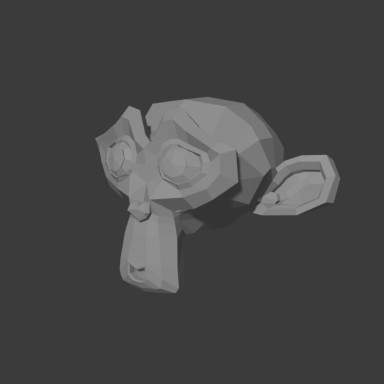
\includegraphics[width=4cm]{figures/monkey/monkey1.jpeg}};
    \node at (3.666,-6) {(1)};
    \draw[->, thick] (2.25,0) -- (3.75,0);

    \node at (6,0) {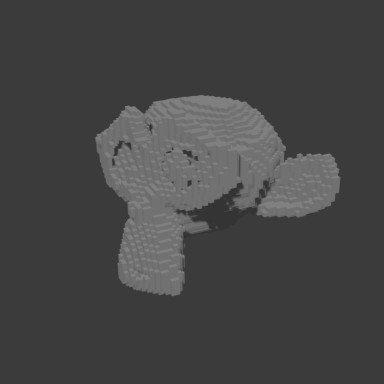
\includegraphics[width=4cm]{figures/monkey/monkey2.jpeg}};
    \node at (9.666,-6) {(2)};

    \node at (12,0) {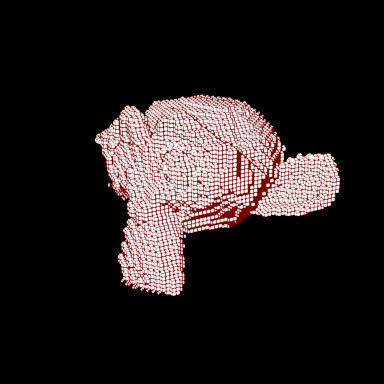
\includegraphics[width=4cm]{figures/monkey/monkey3.jpeg}};
    \node at (15.666,-6) {(3)};

\end{tikzpicture}
    \caption\centering{
        Вокселізація та мапування полігональної моделі в загальний об'єм:\\1 --- полігональна модель;\\2 --- вокселізована модель;\\3 --- представлення у загальному об'ємі (білий --- тверді вокселі, чорний --- порожні; червоною сіткою виділено окремі вокселі).
    }
    \label{fig:monkey}
\end{figure}

В нашому випадку, оскільки сама графіка у нашому застосунку є воксельною, представлення всієї сцени у вигляді загального воксельного об'єму все ще дає нам наступні переваги:
\begin{itemize}[itemsep=0pt, topsep=0pt, label=$\diamond$]
    \item як і вказано вище, це звільняє нас від потреби власноруч \textit{ефективно} організовувати простір для окремих воксельних моделей, у вигляді збалансованих BVH дерев, складних октодерев тощо, оскільки всі моделі підлягають процесу мапування у загальний об'єм, і доступ до даних всередині них, на відміну від пошуку по дереву, відбувається за константний час за допомогою тривимірного індексу;
    \item можливість використання MIP-рівнів 3D текстури для швидкого пропуску великих порожніх областей простору під час трасування, що аналогічно до переваг октодерева, але без складності його побудови;
    \item єдиний уніфікований простір координат спрощує обчислення взаємодій між об'єктами (тіні, відбиття, ambient occlusion), оскільки всі об'єкти вже знаходяться в одній системі координат без потреби додаткових трансформацій.
\end{itemize}

\section{Постановка задачі}

Метою даної роботи є розробка та дослідження методу рендерингу тривимірних сцен на основі трасування променів у дискретному воксельному просторі з використанням загального світового воксельного об'єму, орієнтованого на виконання на графічному процесорі. Основний акцент робиться не на повній фізичній коректності освітлення, а на досягненні прийнятного балансу між якістю зображення, швидкодією та простотою реалізації, що є критично важливим для інтерактивних застосунків, зокрема ігрових рушіїв та візуалізацій у реальному часі.

У межах роботи передбачається, що всі об'єкти сцени — як спочатку воксельні, так і полігональні — проходять етап вокселізації та мапуються в єдиний світовий воксельний об'єм фіксованої роздільної здатності. Цей об'єм зберігається у вигляді 3D-текстури з MIP-рівнями та використовується як основне джерело даних для алгоритму трасування променів. Таким чином, задача трасування зводиться до ефективного проходження дискретного простору та визначення перетинів променя з твердими вокселями.

В рамках поставленої мети необхідно розв'язати такі основні задачі:

\begin{itemize}[itemsep=0pt, topsep=0pt, label=$\diamond$]
\item спроєктувати модель представлення світового воксельного об'єму, придатну для зберігання на GPU, з урахуванням обмежень шейдерних мов та обсягу відеопам'яті;
\item розробити алгоритм мапування (вокселізації) окремих об'єктів сцени у спільний дискретний простір, включно з підтримкою трансформацій (зміщення, обертання, масштабування);
\item реалізувати алгоритм трасування променів у воксельному просторі на основі інкрементального проходження (DDA або подібного підходу), адаптований до дискретної природи даних;
\item дослідити та врахувати характерні числові та геометричні проблеми такого підходу, зокрема явища тіньового та «екстремального» тіньового акне, та запропонувати практичні способи їх усунення;
\item використати MIP-рівні 3D-текстури як наближену форму ієрархії простору для прискорення трасування шляхом пропуску великих порожніх ділянок;
\item забезпечити коректну роботу з буфером глибини для підтримки перекривання об'єктів та поєднання результатів трасування з іншими етапами рендерингу.
\end{itemize}

Окремою задачею є визначення меж застосовності запропонованого підходу. Зокрема, необхідно врахувати, що розмір одиничного вокселя безпосередньо впливає як на візуальну точність, так і на споживання пам'яті та продуктивність. Тому в роботі приймається припущення, що сцена має обмежені розміри або ж може бути розбита на окремі чанки, які підвантажуються та обробляються незалежно. Також допускається спрощене представлення властивостей матеріалів вокселів (наприклад, без повноцінної підтримки глобального освітлення), якщо це дозволяє суттєво зменшити складність реалізації.

У результаті виконання роботи очікується отримання прототипу рендереру, який:

\begin{itemize}[itemsep=0pt, topsep=0pt, label=$\diamond$]
\item демонструє можливість використання єдиного світового воксельного \linebreak об'єму як універсальної структури даних для трасування променів;
\item забезпечує стабільну роботу в реальному часі для сцен середньої складності;
\item може бути розширений у майбутньому за рахунок додавання більш складних моделей освітлення, матеріалів або динамічних змін сцени.
\end{itemize}